\documentclass[red]{beamer}
\usetheme{Madrid}
%\usepackage{caption}
%\DeclareCaptionType{copyrightbox}
\graphicspath{{../figures/}}
% \usepackage{subcaption}
% \captionsetup{compatibility=false}
\usepackage{subfig}
\usepackage{graphicx}
\usepackage{multirow}
\usepackage{amsmath, amsfonts, amssymb}
\usepackage[utf8]{inputenc}
\inputencoding{utf8}

\newcommand{\then}{\Rightarrow}
\newcommand{\softor}{\operatornamewithlimits{\tilde{\vee}}}
\newcommand{\softand}{\operatornamewithlimits{\tilde{\wedge}}}
\newcommand{\softthen}{\operatornamewithlimits{\tilde{\then}}}
\newcommand{\softneg}{\operatornamewithlimits{\tilde{\neg}}}


\begin{document}

\title[Planned Protest]{Forecasting Protests by Detecting Future Time Mentions in News and Social Media
}
\author{Sathappan Muthiah}
\institute{Virginia Tech}
\date{July 2nd, 2014}
\subject{Computer Science}


\frame{\titlepage}



%Table of Contents slide
\begin{frame}
\frametitle{Table of Contents}
\tableofcontents
\end{frame}
\section{Problem Overview}
\begin{frame}
\frametitle{Table of Contents}
\tableofcontents[currentsection]
\end{frame}


\begin{frame}
    \frametitle{Problem Overview}
    \begin{itemize}
        \item
            Detecting Future time mentions in relevant media to build a protest forecasting system
        \item
            Investigate the selective superiorities of different social media
    \end{itemize}
\end{frame}

\subsection{motivation}
\begin{frame}
    \frametitle{Motivation}
    \begin{itemize}
        \item
            Around 75\% of the protests are planned, organized, or announced in advance
        \item
            Identifying these planned protests is an easy way to forecast protests
    \end{itemize}
\end{frame}


\begin{frame}
    \frametitle{Key Contributions}
    \begin{itemize}
        \item
            Real-Time Prospective Study - most studies until now have been retrospective
        \item
            Semi-Automatic approach for learning keyphrase filters
        \item
            Handling mutliple sources
        \item
            Reasoning about locations
        \item
            Handling relative dates - some recent work use only absolute dates
    \end{itemize}
\end{frame}


\begin{frame}
\frametitle{Overall Framework}
\begin{figure}
    \centering
    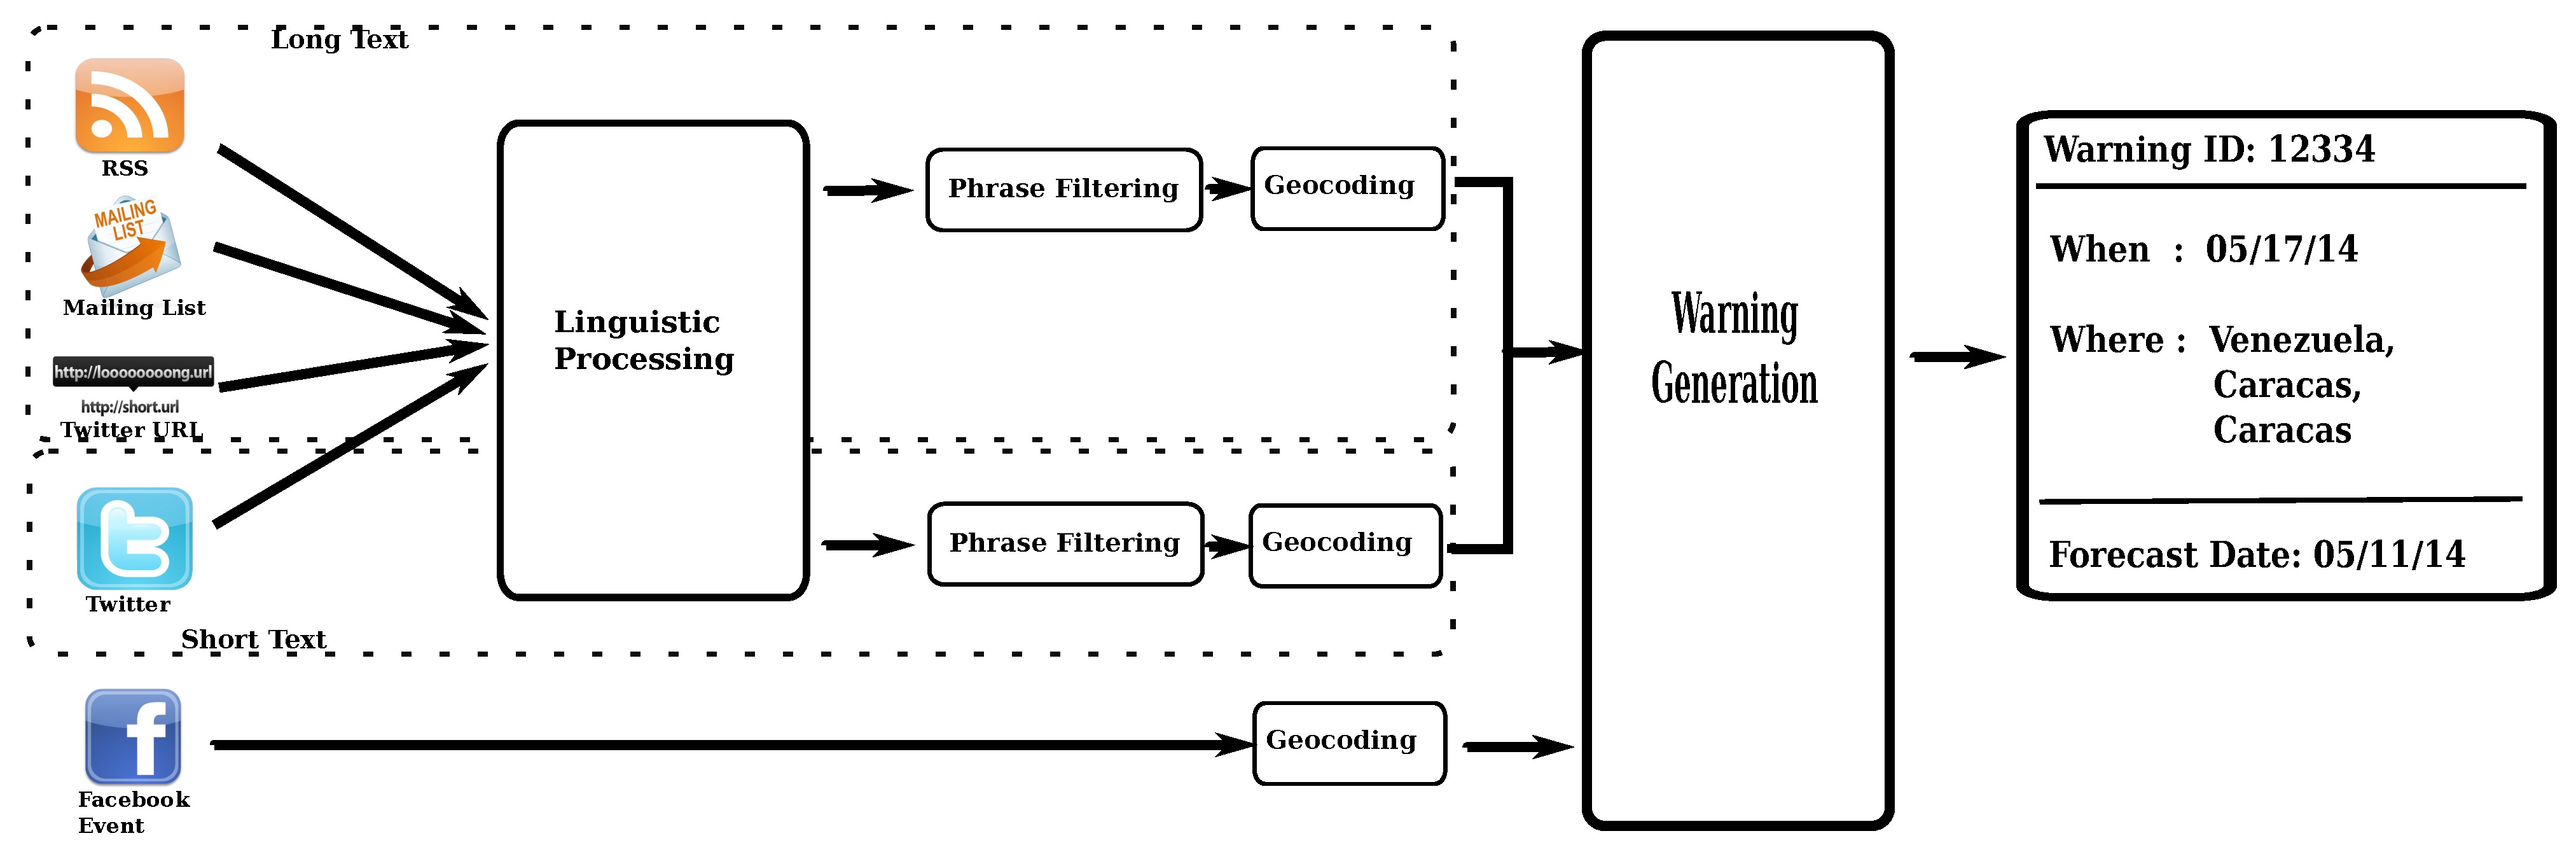
\includegraphics[height=0.6\textheight,width=\textwidth]{pipeline}
\end{figure}
\end{frame}


\section{Data Sources}

\begin{frame}
\frametitle{Table of Contents}
\tableofcontents[currentsection]
\end{frame}
\begin{frame}
    \frametitle{Data Sources}
    \begin{itemize}
        \item
            Long Text
            \begin{itemize}
                \item
                    RSS Feeds
                    \begin{itemize}
                        \item
                            News
                        \item
                            Blogs
                    \end{itemize}
                \item
                    Twitter-URL
            \end{itemize}
        \item
            Short Text
                \begin{itemize}
                    \item
                        Twitter
                \end{itemize}
        \item
            Facebook-Event

    \end{itemize}
\end{frame}


\begin{frame}
    \frametitle{Long Text - RSS Feeds}
    \begin{itemize}
        \item
            A total of 9498 different RSS feeds are ingest - 6236 news sources and 3262 blogs
        \item
            Duration: November 2012 to present
        \item
            List of news sources to ingest were obtained from Wikipedia,\url{www.onlinenewspapers.com}, LANIC, etc
        \item
            List of blogs were obtained from blog search engines like \url{www.technorati.com}
        \item
            Google/Talkwalker Alerts - Alerts for phrases in our keyphrase dictionary
    \end{itemize}
\end{frame}

\begin{frame}
    \frametitle{Long Text - Example}

   \begin{columns}
       \column{0.3\textwidth}
       \hspace{-1em}
       \begin{figure}
           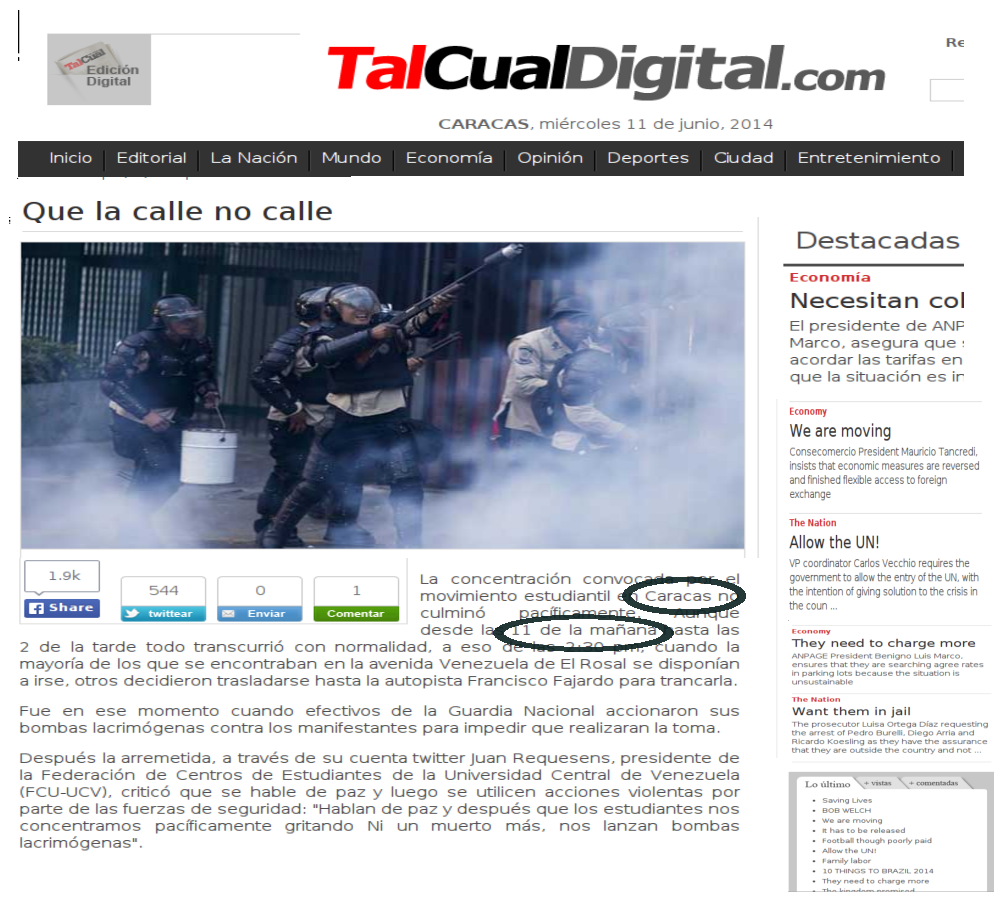
\includegraphics[scale=0.27]{pp_example}
       \end{figure}
       \column{0.5\textwidth}
       \begin{figure}
           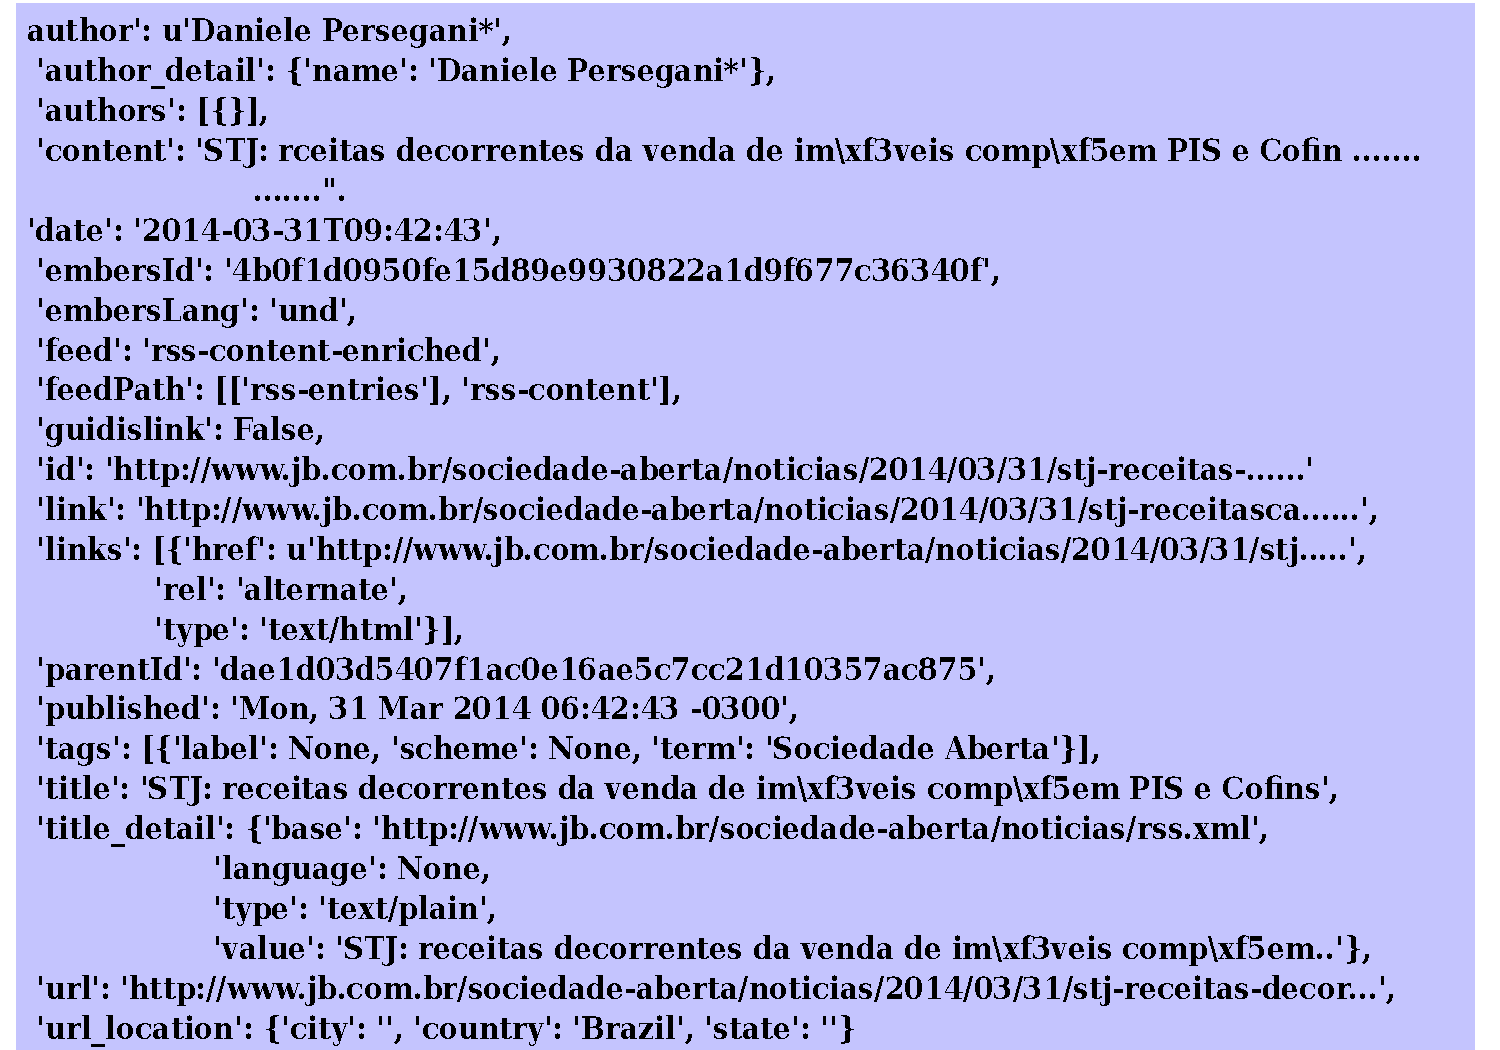
\includegraphics[scale=0.27]{rss_example}
       \end{figure}
   \end{columns}
\end{frame}

\begin{frame}
    \frametitle{Short Text - Twitter}
        \begin{itemize}
            \item
                Datasift Firehose
            \item
                Duration: November 2012 to present
            \item
                URL's mentioned in a tweet are fetched and used as a separate source (alongwith RSS feeds).
        \end{itemize}
\end{frame}

\iffalse
\begin{frame}
    \frametitle{Example}
\end{frame}
\fi

\begin{frame}
    \frametitle{Facebook}
    \begin{columns}
        \column{0.3\textwidth}
    \begin{itemize}
        \item
            Facebook Graph API - Query for Facebook Events that contain a particular keyword
        \item
            Facebook Query Language (FQL) - Obtain extra information of an Event-Id obtained by searching through Graph API
    \end{itemize}
    \column{0.4\textwidth}
    \begin{figure}
        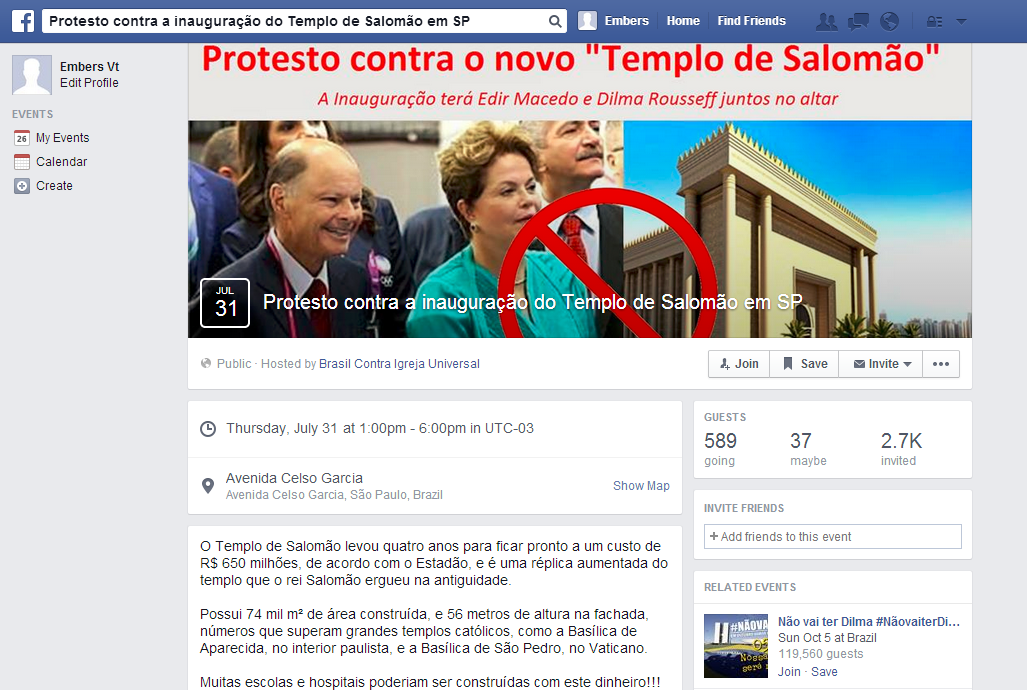
\includegraphics[scale=0.22]{FB_Event_example}
    \end{figure}
    \end{columns}
\end{frame}

\section{Preliminaries}
\begin{frame}
\frametitle{Table of Contents}
\tableofcontents[currentsection]
\end{frame}
\begin{frame}
\frametitle{Preliminaries-Probabilistic Soft Logic}
    \begin{itemize}
        \item
            Framework for collective probabilistic reasoning in relational domains
        \item
            Uses first order logic rules as a template language for graphical models
        \item
            Soft truth values
        \item
            Applications in collective classification, ontology alignment,opinion diffusion, graph summarization etc
        \item
            A simple PSL rule:
            \begin{figure}
                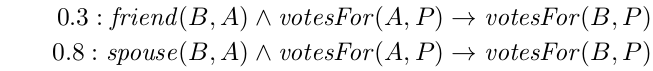
\includegraphics[scale=0.3]{psl_rule_example}
            \end{figure}
    \end{itemize}
\end{frame}

\begin{frame}
    \frametitle{PSL MPE Inference}
    \begin{itemize}
        \item Lukasiewicz t-norm is used to determine the degree to which a ground rule is satisfied
        \item Most Probable Explanation or Inference (MPE): Inferring the most likely values for a proposition given values of remaining propositions
            \begin{figure}
                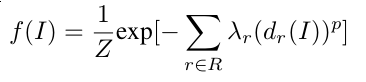
\includegraphics[scale=0.4]{psl_equation}
            \end{figure}
        \item Here,
            $I$ is an interpretation of the proposition,

            $\lambda_r$ is the weight of the rule,

            $d_r(I)$ is the distance to satisfaction of the rule (degree to which the condition/rule is violated)
        \end{itemize}
\end{frame}

\section{Linguistic Preprocessing}
\begin{frame}
\frametitle{Table of Contents}
\tableofcontents[currentsection]
\end{frame}
\subsection{Natural Language Enrichment}
\begin{frame}
    \frametitle{Natural Language Enrichment}
    \begin{columns}
        \column{0.4\textwidth}
            \begin{itemize}
                \item
                    Tokenization
                \item
                    Lemmatization
                \item
                    Noun Phrase Extraction
                \item
                    Named Entity Extraction and Classification
            \end{itemize}
        \column{0.4\textwidth}
        \begin{figure}
            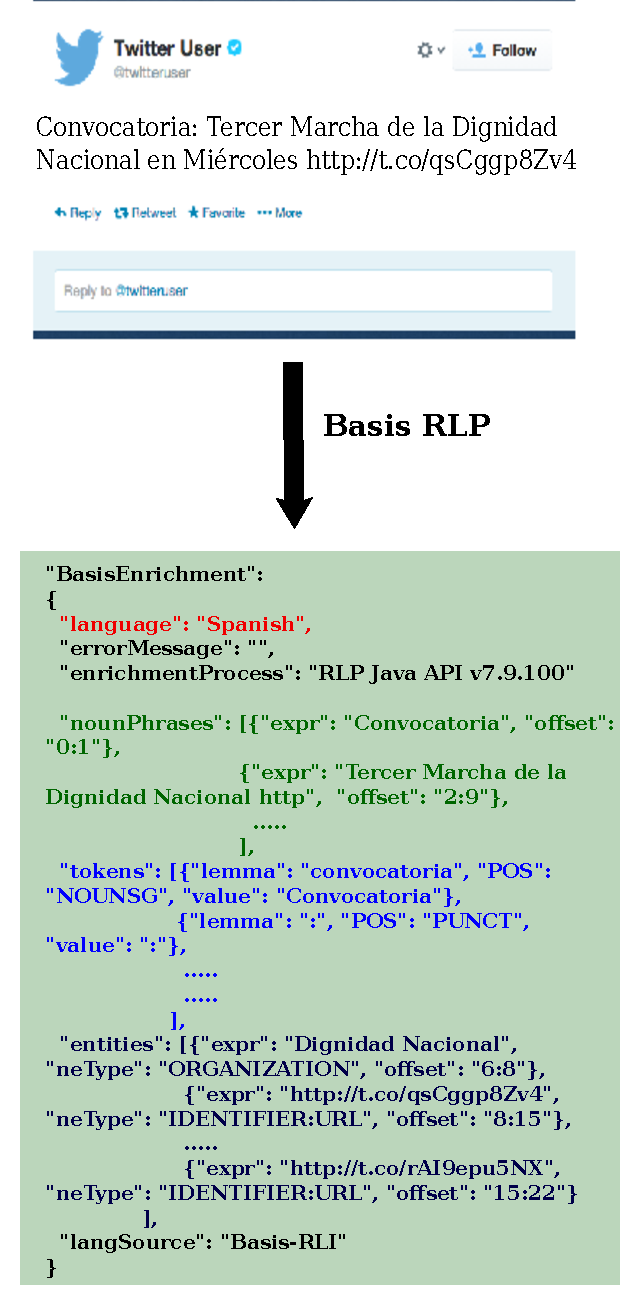
\includegraphics[scale=0.3]{basis_enrichment}
        \end{figure}
    \end{columns}
\end{frame}

\subsection{TIMEN Enrichment}
\begin{frame}
\frametitle{TIMEN Enrichment}
    \begin{columns}
        \column{0.4\textwidth}
        \begin{itemize}
            \item
                Extraction of Absolute Dates from text
            \item
                Identification of Relative dates like `yesterday, next wednesday' etc
        \end{itemize}
        \column{0.4\textwidth}
        \begin{figure}
            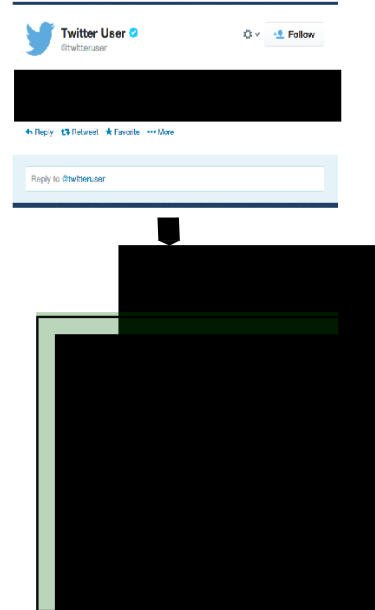
\includegraphics[scale=0.4]{timen_enrichment}
        \end{figure}
    \end{columns}
\end{frame}

\section{Geocoding}
\begin{frame}
\frametitle{Table of Contents}
\tableofcontents[currentsection]
\end{frame}
\subsection{RSS}
\begin{frame}
\frametitle{Geocoding - RSS Feeds}
\begin{figure}
    \centering
    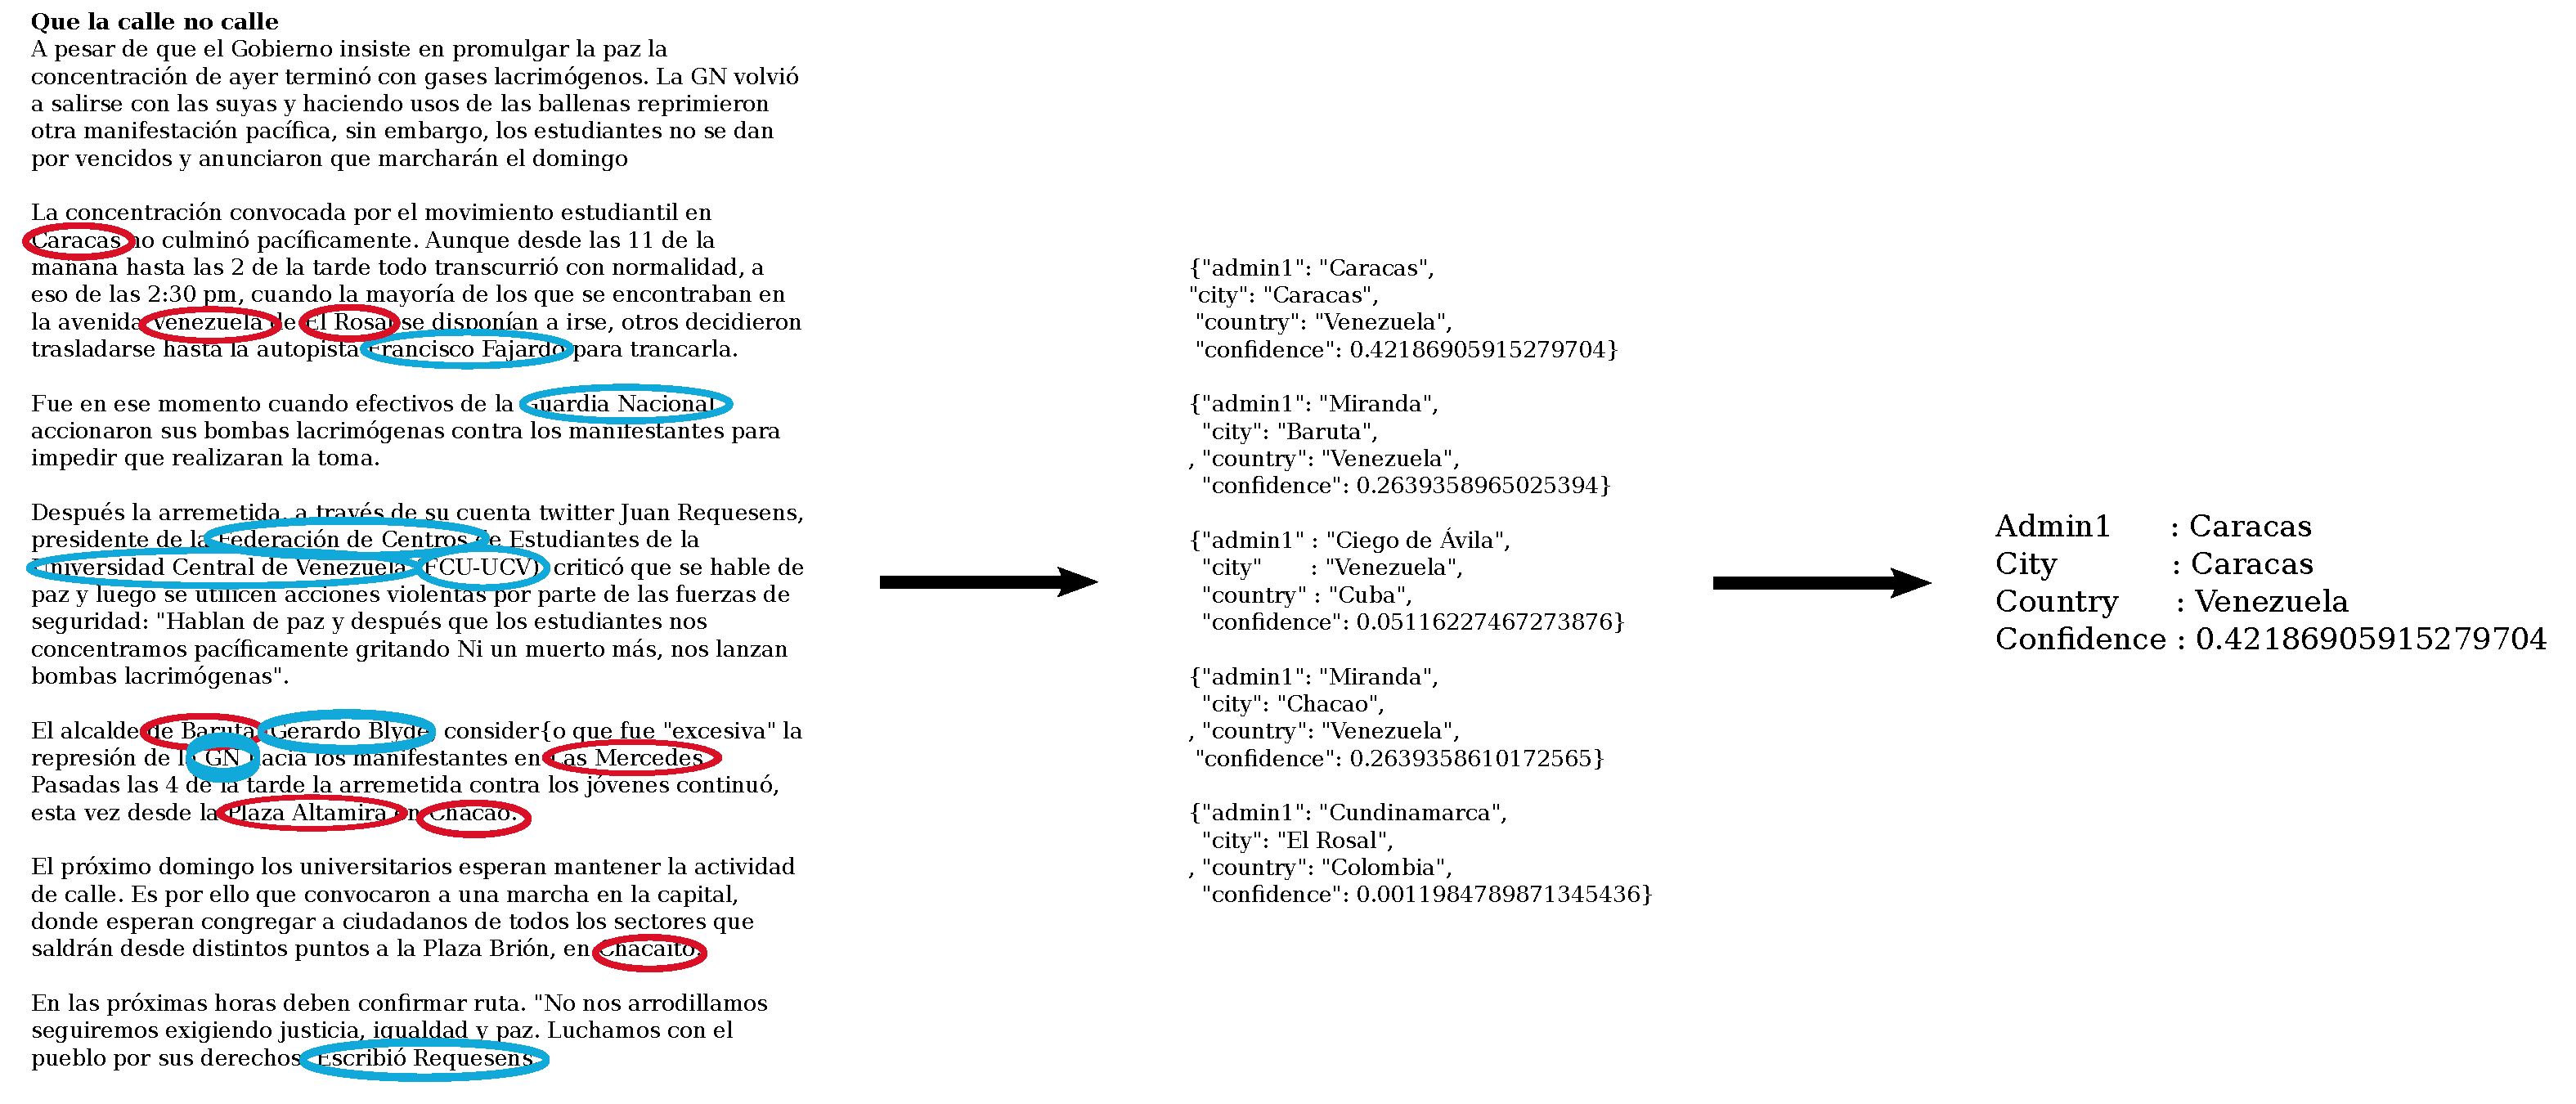
\includegraphics[width=\textwidth]{psl_pipeline2}
\end{figure}
\end{frame}

\begin{frame}
    \frametitle{Geocoding - RSS Feeds (contd...)}
    \begin{itemize}
        \item Primary rules
        \begin{flalign*}
            ENTITY&(L, location) \softand REFERSTO(L, locID) &\\
                                &\rightarrow PSLLOCATION(Article, locID) &
        \end{flalign*}


        \begin{flalign*}
            ENTITY&(C, location) \softand IsCountry(C) &\\
                                &\rightarrow ArticleCountry(Article, C) &
        \end{flalign*}


        \begin{flalign*}
            ENTITY&(S, location) \softand IsState(S)&\\
                                    &\rightarrow ArticleState(Article, S)&
        \end{flalign*}

    \end{itemize}
\end{frame}

\begin{frame}
    \frametitle{Geocoding - RSS Feeds (contd...)}
    \begin{itemize}
        \item Secondary rules
    \begin{flalign*}
        ENTITY&(O, organization) \softand REFERSTO(O, locID)&\\
                                &\rightarrow PSLLOCATION(Article, locID) &
    \end{flalign*}


    \begin{flalign*}
        ENTITY&(O, organization) \softand IsCountry(O)&\\
            &\rightarrow ArticleCountry(Article, O)&
    \end{flalign*}


    \begin{flalign*}
        ENTITY&(O, organization) \softand IsState(O)&\\
              &\rightarrow ArticleState(Article, O) &
    \end{flalign*}

    \end{itemize}
\end{frame}

\subsection{Twitter}
\begin{frame}
\frametitle{Geocoding - Twitter}
    \begin{itemize}
        \item
            Geotag of the tweet
        \item
            Twitter ``places" metadata
        \item
            Other text fields (user profile, tweet text)
    \end{itemize}
\end{frame}

\subsection{Facebook}
\begin{frame}
\frametitle{Geocoding - Facebook}
    \begin{itemize}
        \item
            Facebook Locations - similar to twitter places
        \item
            Facebook Event Venue tag
        \item
            Nearest geocoded point search using KD-Tree algorithm
    \end{itemize}
\end{frame}

\section{Phrase Filtering}
\begin{frame}
\frametitle{Table of Contents}
\tableofcontents[currentsection]
\end{frame}

\subsection{Phrase List Development}
\begin{frame}
\frametitle{Phrase List Development}
    \begin{itemize}
        \item
            Semi-Automatic
        \item
            Different Lists are built for different Sources
        \item
            Seed phrases are identified from analysis of known planned events from print media.
    \end{itemize}

\end{frame}

\subsection{Dependency Parsing}
\begin{frame}
    \frametitle{Dependency Parsing}
    \begin{figure}
        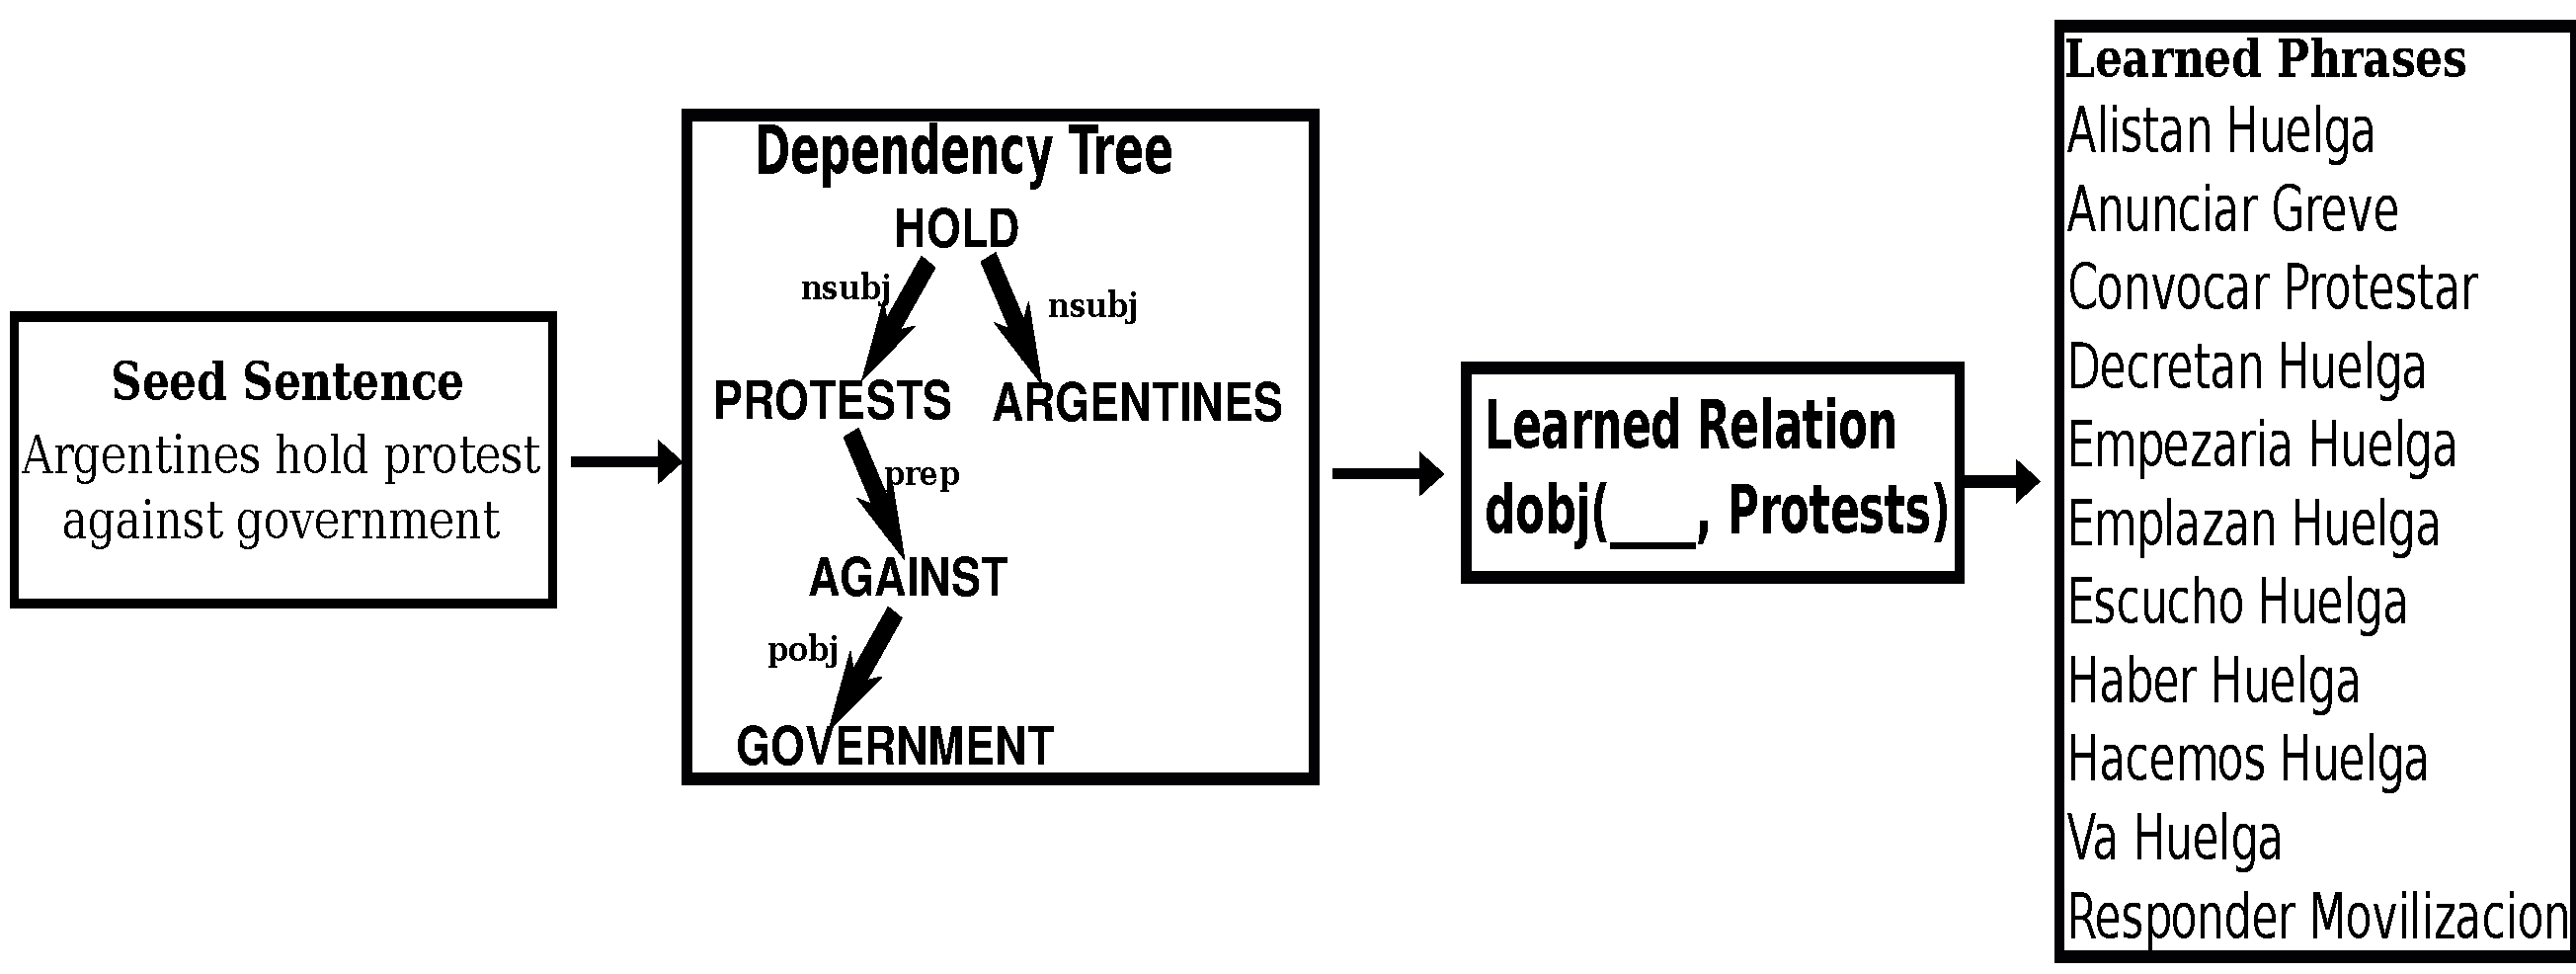
\includegraphics[width=\textwidth]{phraseLearning}
    \end{figure}
\end{frame}

\subsection{Examples}
\begin{frame}
    \frametitle{Phrase List for Long Text}
    \begin{figure}
        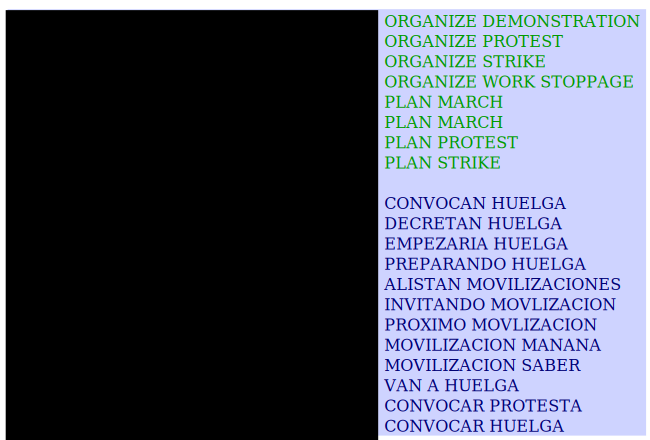
\includegraphics[scale=0.5]{wordlist_rss}
    \end{figure}
\end{frame}


\begin{frame}
    \frametitle{Phrase List for Short text}
     \begin{figure}
        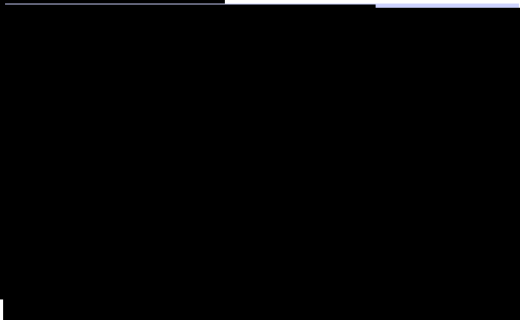
\includegraphics[scale=0.5]{wordlist_twitter}
     \end{figure}
\end{frame}

\subsection{Phrase Matching}
\begin{frame}
    \frametitle{Phrase Matching}
    \begin{itemize}
        \item
            Sample phrase matching rule:
            \begin{figure}
                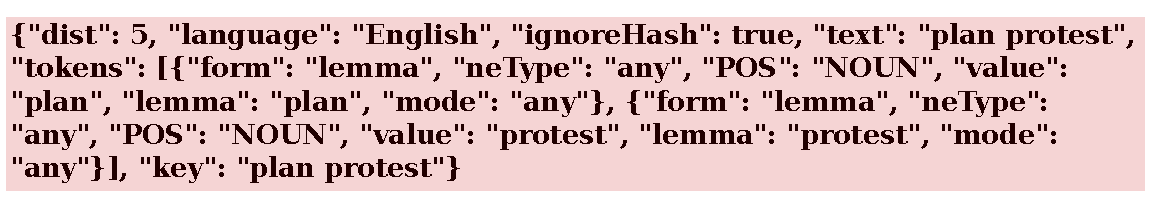
\includegraphics[scale=0.5]{phrase_rule}
            \end{figure}
        \item
            Linguistically sophisticated and flexible matching
        \item
            Near regex style matching
        \item
            Example matched sentence:
            {\em ``The students are planning a couple of big protests tomorrow"}
    \end{itemize}
\end{frame}


\begin{frame}
    \frametitle{System Framework Once again}
    \begin{figure}
        \centering
        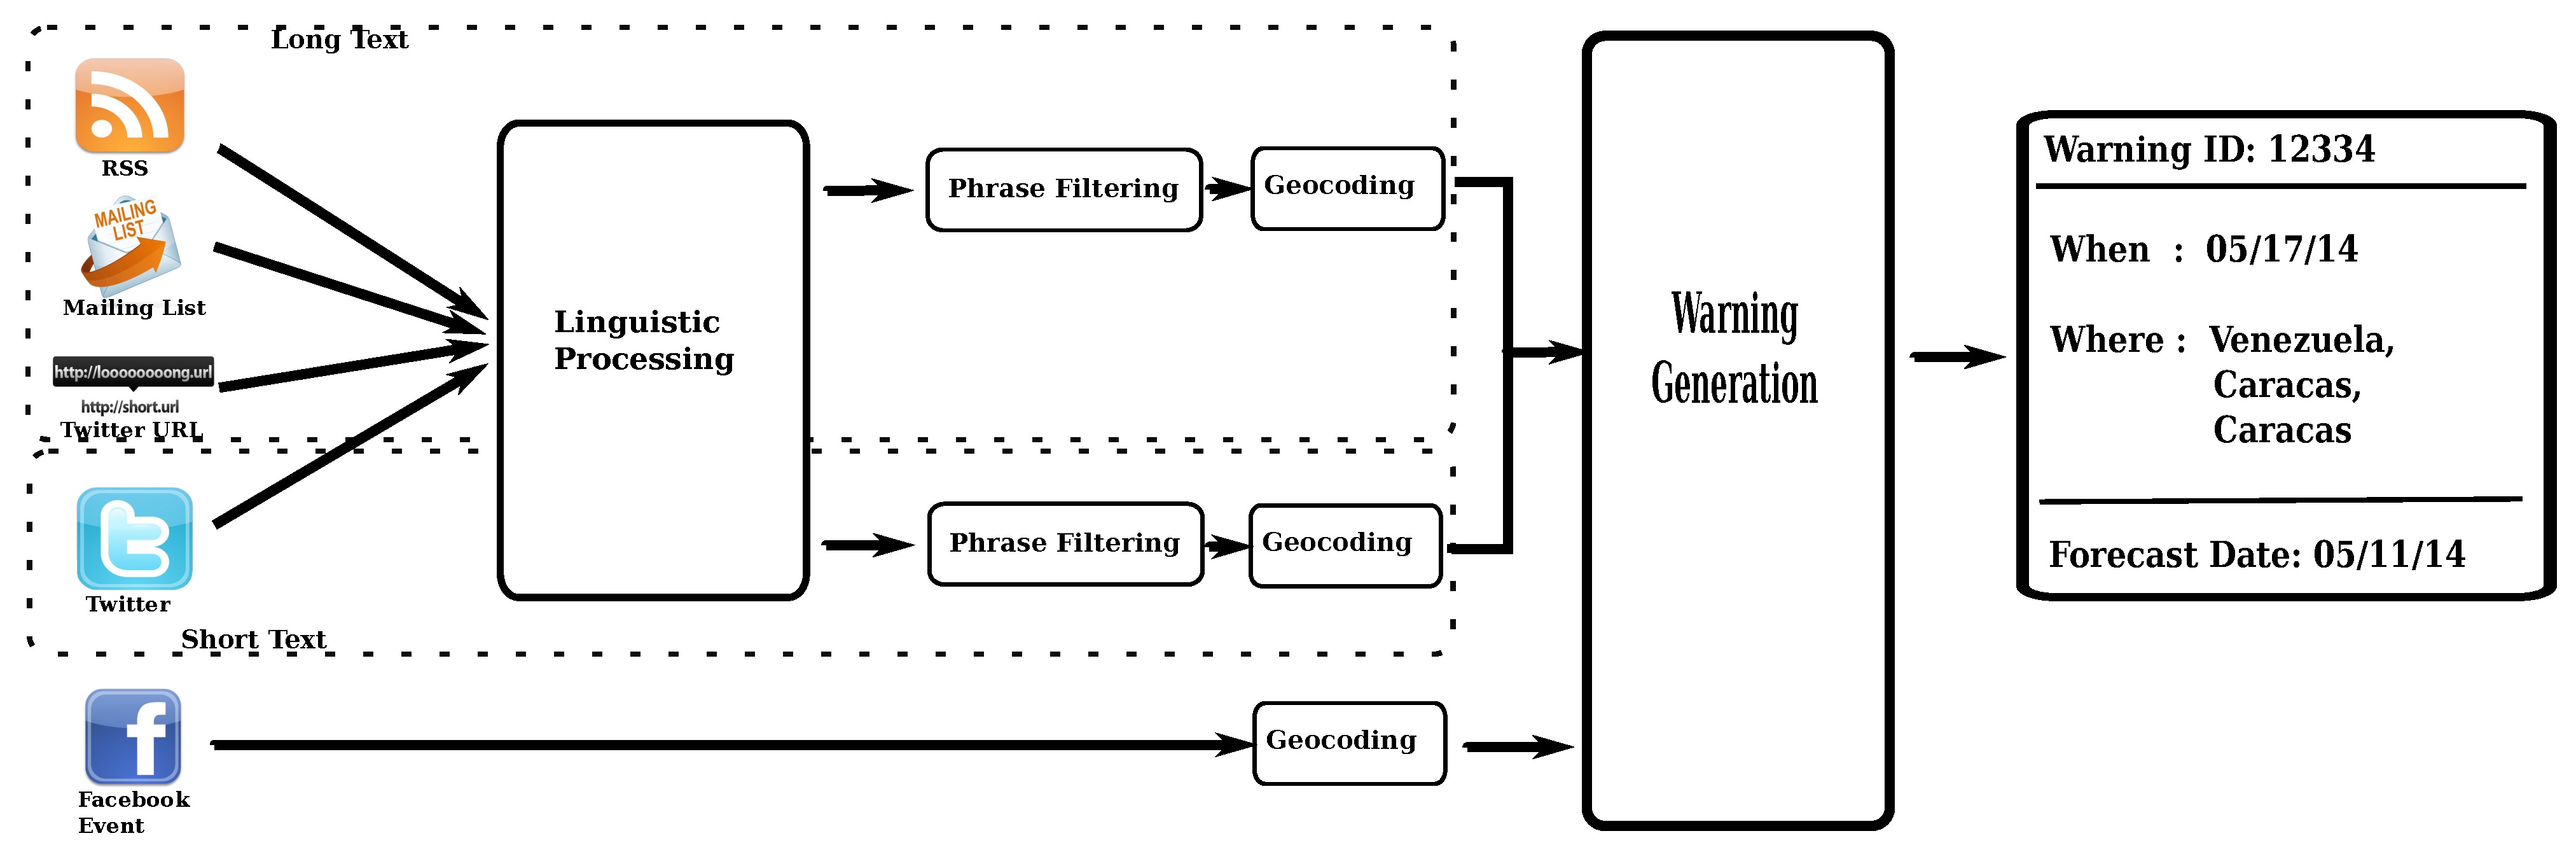
\includegraphics[height=0.6\textheight,width=\textwidth]{pipeline}
    \end{figure}
\end{frame}

\section{Evaluation}
\begin{frame}
\frametitle{Table of Contents}
\tableofcontents[currentsection]
\end{frame}

\subsection{Evaluation Methodology}
\begin{frame}
\frametitle{Evaluation Methodology}
    \begin{itemize}
        \item
            Bipartite Matching
    \end{itemize}
    \begin{figure}
        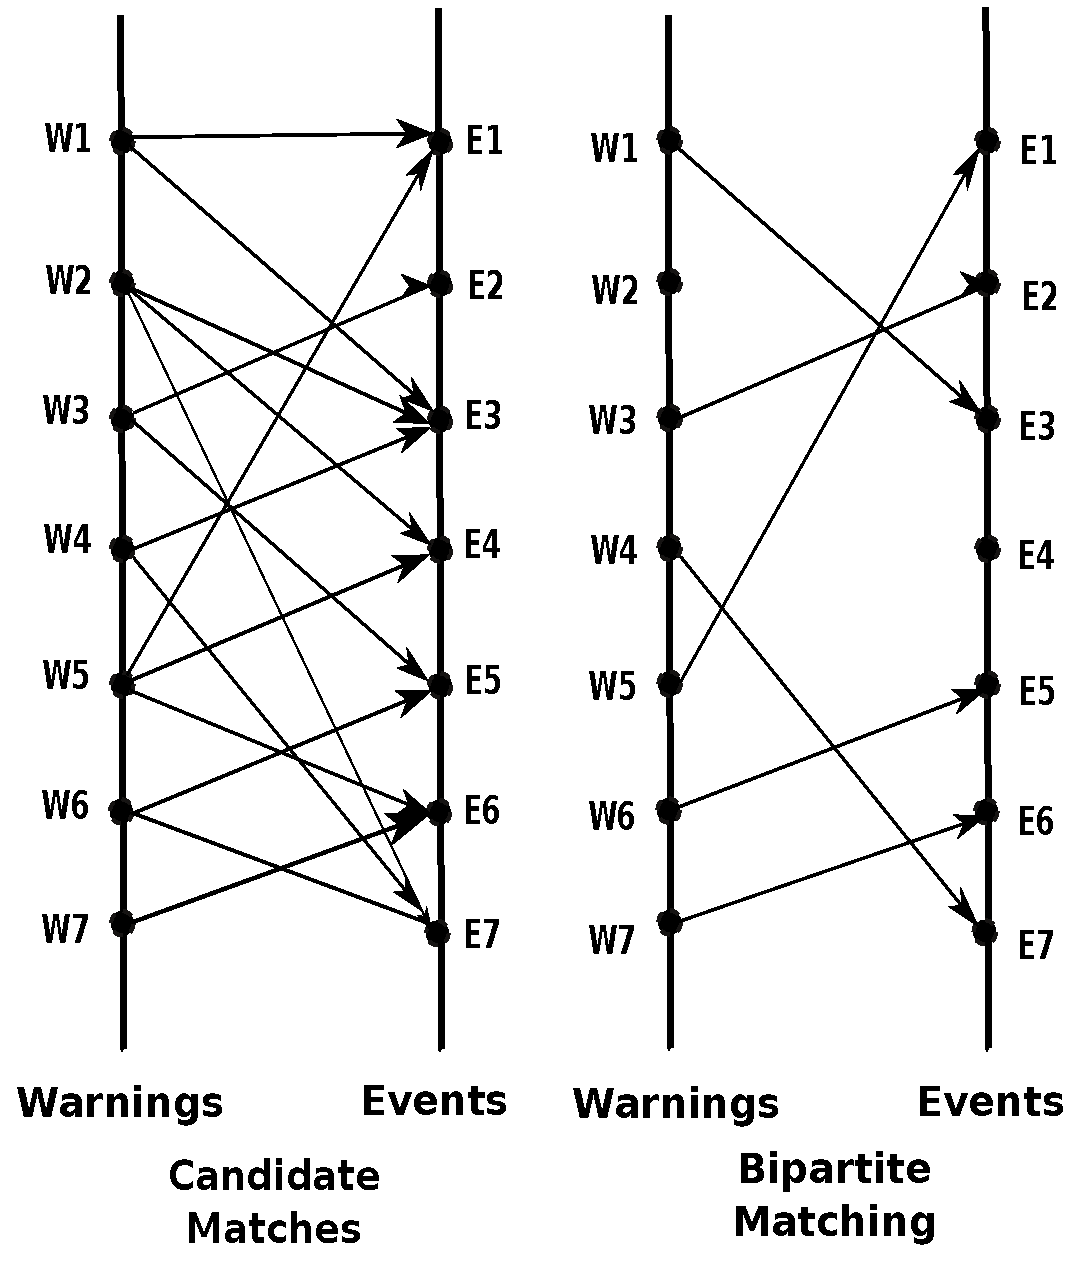
\includegraphics[height=0.7\textheight]{matching}
    \end{figure}

\end{frame}


\begin{frame}
    \frametitle{Evaluation Methodology (contd ...)}
    \begin{itemize}
        \item
            Location Score
            \begin{equation*}
                \operatorname{LS}=1 - \frac{\min(\textrm{distance offset}, 300)}{300}
            \end{equation*}
        \item
            Date Score
            \begin{equation*}
                \operatorname{DS}=1 - \frac{\min(\textrm{date offset}, \operatorname{INTERVAL})}{\operatorname{INTERVAL}}
            \end{equation*}

        \item
            Total Quality Score
            \begin{equation*}
                \operatorname{QS}=(\operatorname{DS} + \operatorname{LS})*2
            \end{equation*}
    \end{itemize}

\end{frame}

\begin{frame}
    \frametitle{Warnings vs GSR}
    \begin{figure}%
    \centering
    \subfloat{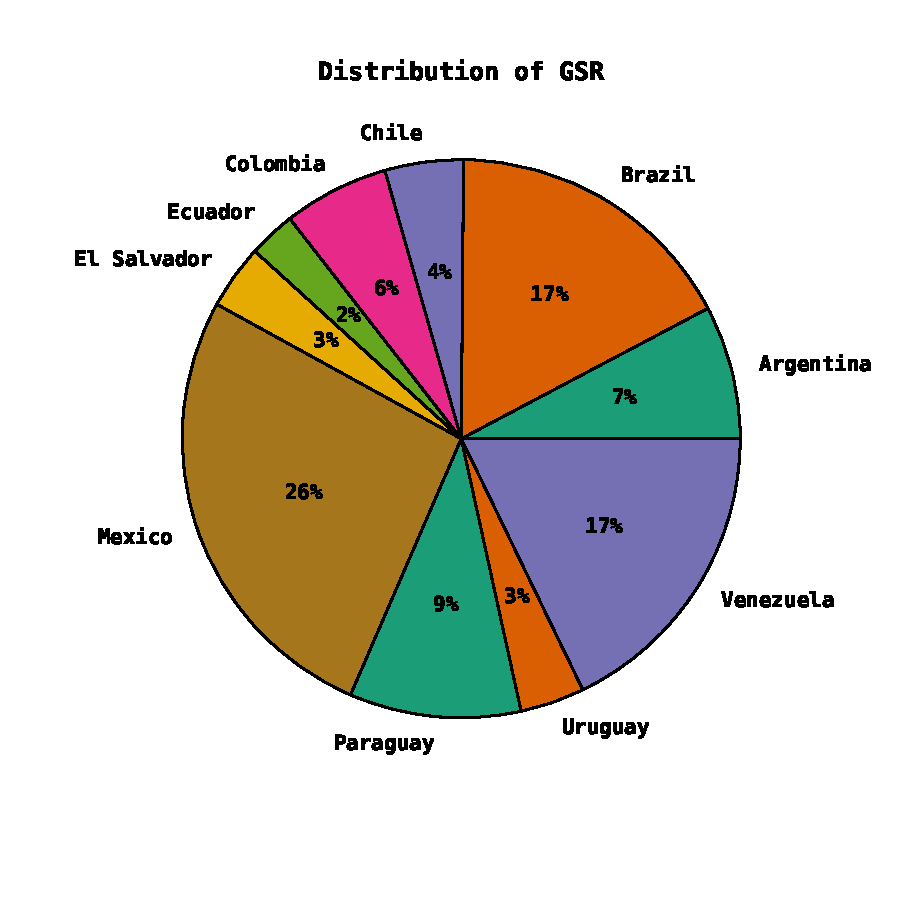
\includegraphics[width=0.45\textwidth]{gsr_distribution}}%
    \qquad
    \subfloat{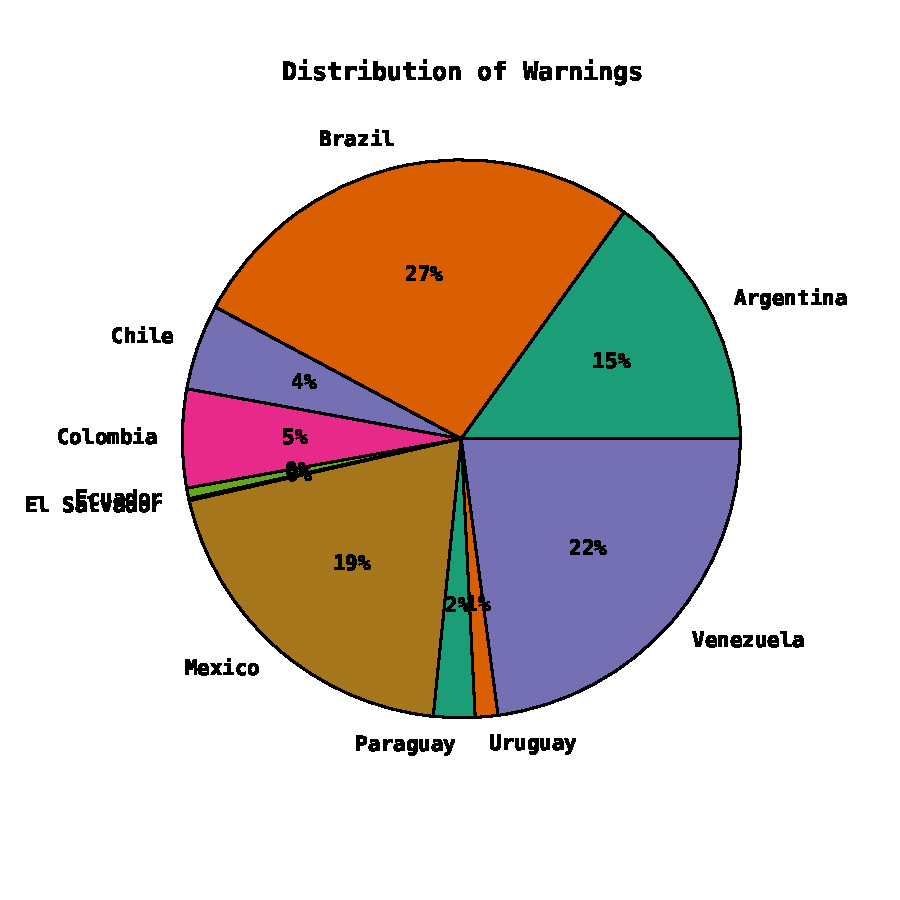
\includegraphics[width=0.45\textwidth]{pp_dist}}%
    \end{figure}
\end{frame}

\begin{frame}
     \frametitle{Venezuelan Spring}
     \begin{figure}
        \centering
        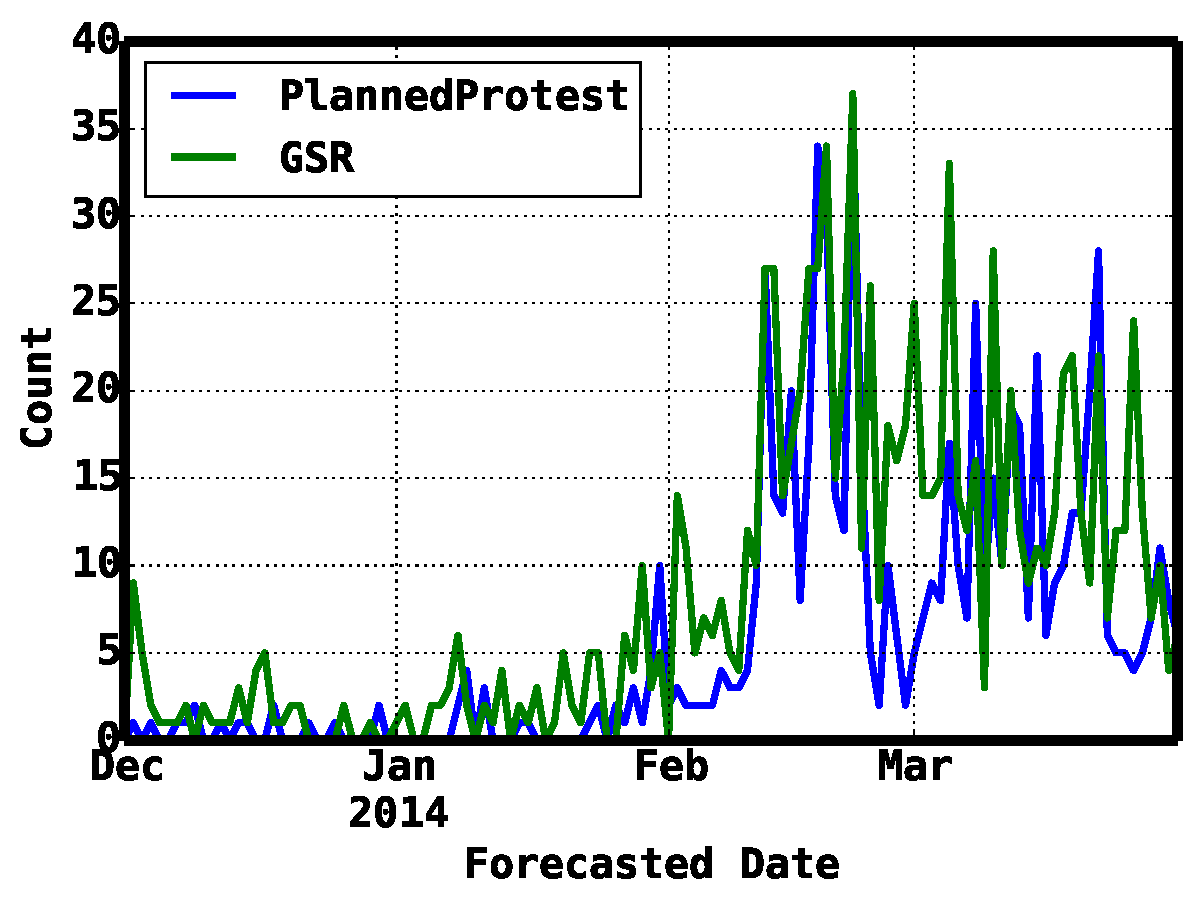
\includegraphics[scale=0.4]{venezuela}
     \end{figure}
\end{frame}

\begin{frame}
    \frametitle{Venezuelan Violent Protests}
     \begin{figure}
        \centering
        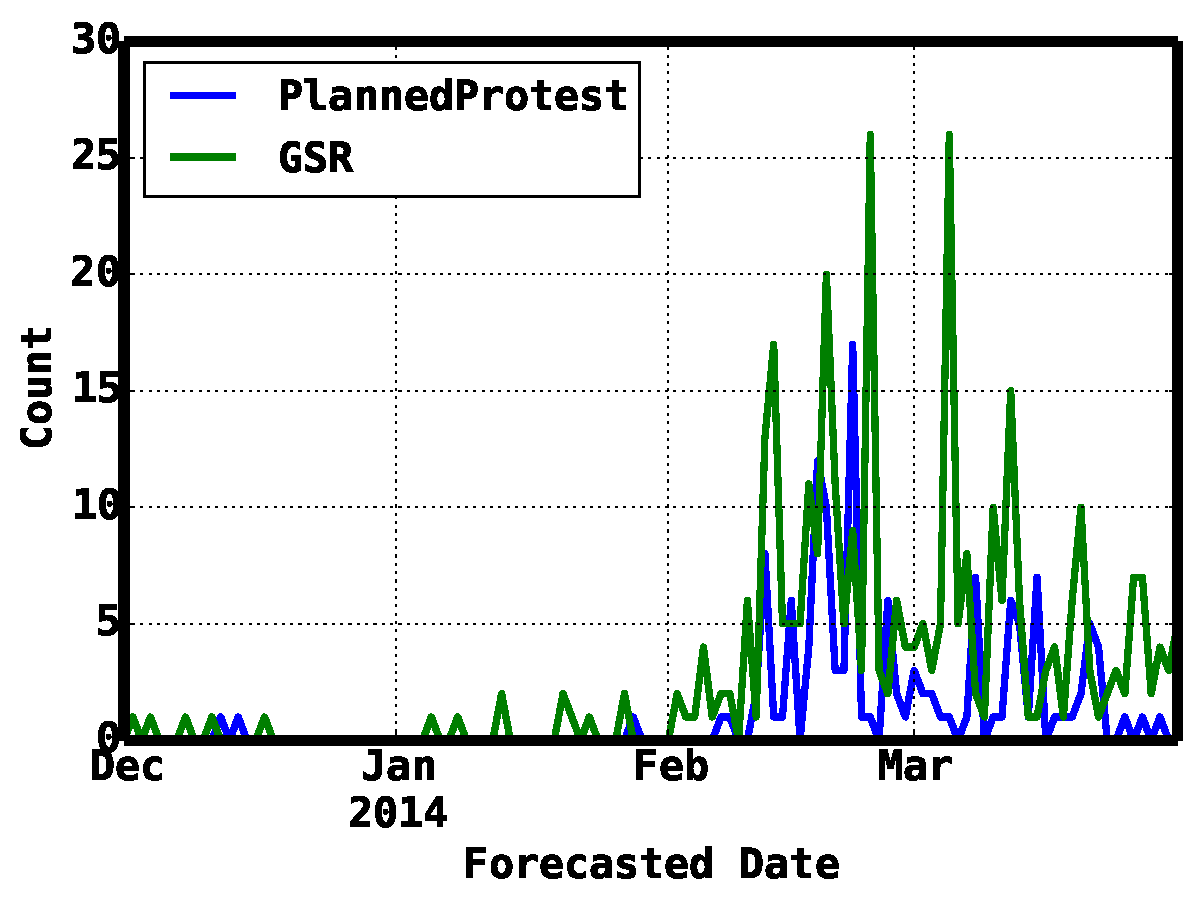
\includegraphics[scale=0.4]{venezuela_violent}
     \end{figure}
\end{frame}

\begin{frame}
    \frametitle{Brazilian Spring}
    \begin{figure}
        \centering
        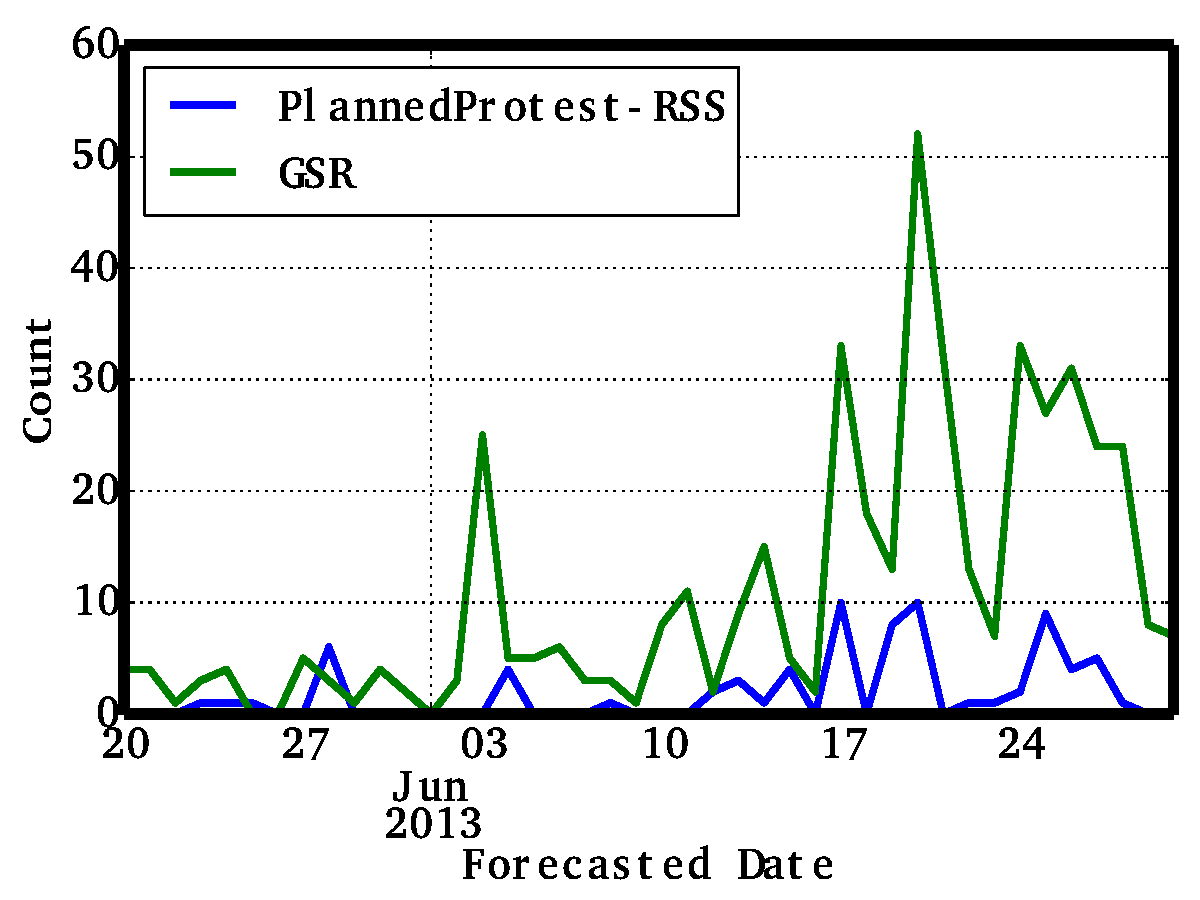
\includegraphics[scale=0.4]{brazil_june}
    \end{figure}
\end{frame}

\begin{frame}
    \frametitle{Individual Source Level Perfomance}
    \resizebox{\linewidth}{!}{
    \begin{tabular}{|*{17}{c|}}
        \hline
        & \multicolumn{4}{ |c| }{News/Blogs} & \multicolumn{4}{ |c| }{Twitter} & \multicolumn{4}{ |c| }{Facebook} & \multicolumn{4}{ |c| }{Combined}\\
        \hline
         & QS & Pr. & Rec. &LT & QS & Pr. & Rec. & LT & QS & Pr. & Rec. & LT & QS & Pr. & Rec. & LT\\
        \hline
        AR &3.14&0.32&0.69&3.94&3.52&{\bf0.78}&0.14&3.14&{\bf3.70}&0.50&0.04&3.00&3.02&0.36&{\bf0.80}&{\bf4.50}\\
        BR &3.14&0.48&0.54&{\bf5.85}&-&-&-&-&{\bf3.62}&{\bf0.76}&0.18&2.46&3.28&0.49&{\bf0.65}&5.15\\
        CL &3.06&0.91&0.67&5.40&{\bf3.52}&{\bf1.00}&0.23&4.29&-&-&-&-&3.16&0.83&{\bf0.80}&{\bf5.92}\\
        CO &2.74&0.90&0.56&{\bf7.44}&3.30&{\bf1.00}&0.15&2.43&{\bf4.00}&{\bf1.00}&0.02&2.00&2.88&0.84&{\bf0.65}&6.47\\
        EC &-&-&-&-&{\bf2.32}&{\bf1.00}&{\bf0.06}&{\bf17.00}&-&-&-&-&{\bf2.32}&{\bf0.50}&{\bf0.06}&{\bf17.00}\\
        MX &2.96&0.88&0.25&{\bf3.69}&3.14&{\bf1.00}&0.02&1.43&{\bf3.72}&0.67&0.01&2.00&3.00&0.87&{\bf0.27}&3.51\\
        SV &{\bf3.22}&{\bf1.00}&{\bf0.03}&{\bf1.0}&-&-&-&-&-&-&-&-&{\bf3.22}&{\bf1.0}&{\bf0.03}&{\bf1.0}\\
        PY &3.38&{\bf1.00}&{\bf0.16}&9.11&3.84&{\bf1.00}&0.04&{\bf11.40}&3.96&{\bf1.00}&0.01&2.00&3.60&0.96&{\bf0.20}&9.35\\
        UY &{\bf3.24}&{\bf1.00}&{\bf0.29}&{\bf2.40}&-&-&-&-&-&-&-&-&3.24&{\bf1.00}&{\bf0.29}&3.24\\
        VE &{\bf3.80}&{\bf1.00}&0.36&{\bf3.27}&3.68&0.97&0.33&2.39&-&-&-&-&3.64&0.99&{\bf0.69}&2.88\\
        ALL &3.34&0.69&0.35&{\bf4.57}&3.62&{\bf0.97}&0.15&2.82&3.66&0.74&0.03&2.44&3.36&0.73&{\bf0.51}&4.08\\
        \hline
    \end{tabular}}
\end{frame}
\iffalse
\begin{frame}
    \frametitle{RSS Feeds + Twitter-Urls}
\end{frame}

\begin{frame}
    \frametitle{Twitter}
\end{frame}

\begin{frame}
    \frametitle{Facebook}
\end{frame}

\begin{frame}
    \frametitle{all Sources}
\end{frame}
\fi
\begin{frame}
    \frametitle{Performance over time}
    \begin{figure}
        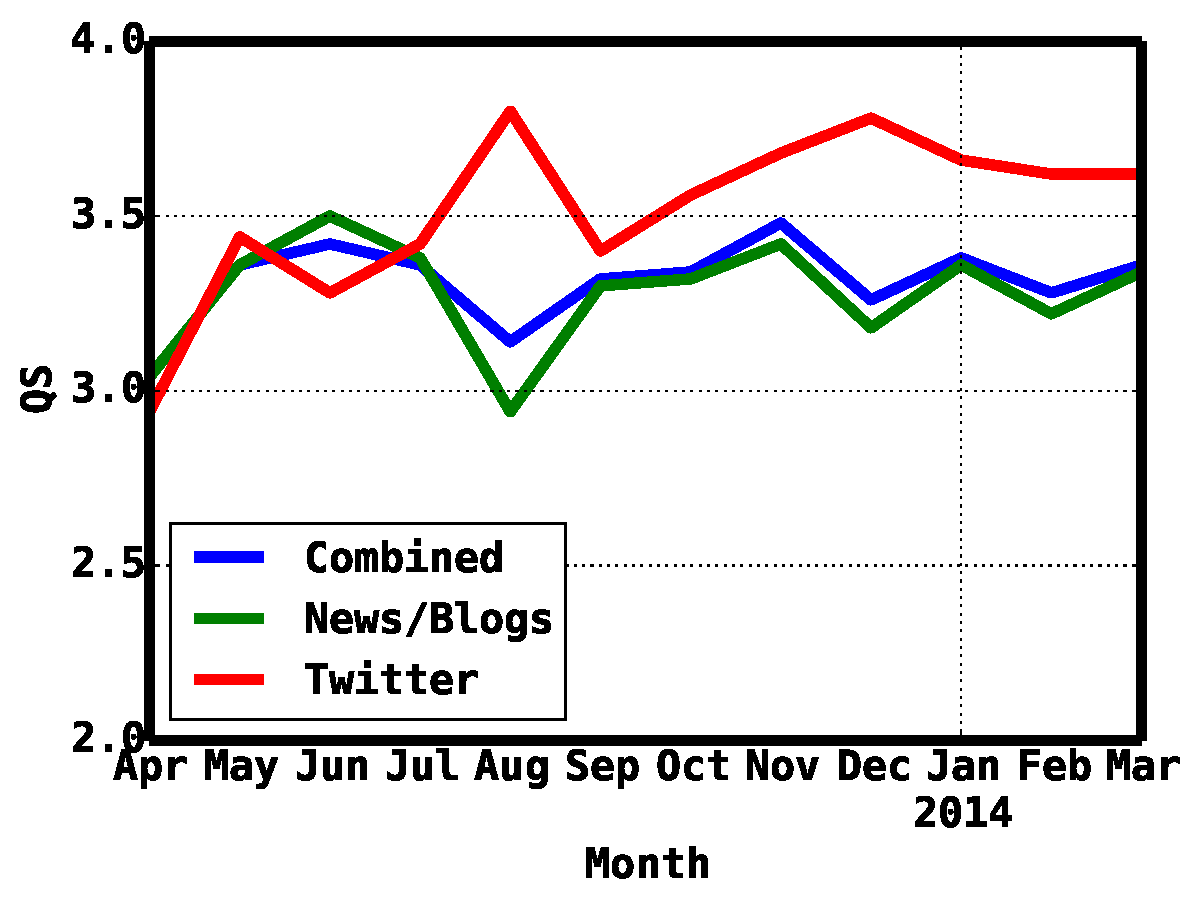
\includegraphics[scale=0.4]{monthlyqs}
    \end{figure}
\end{frame}

\begin{frame}
    \frametitle{Quality Score vs Matching window size}
    \begin{figure}
        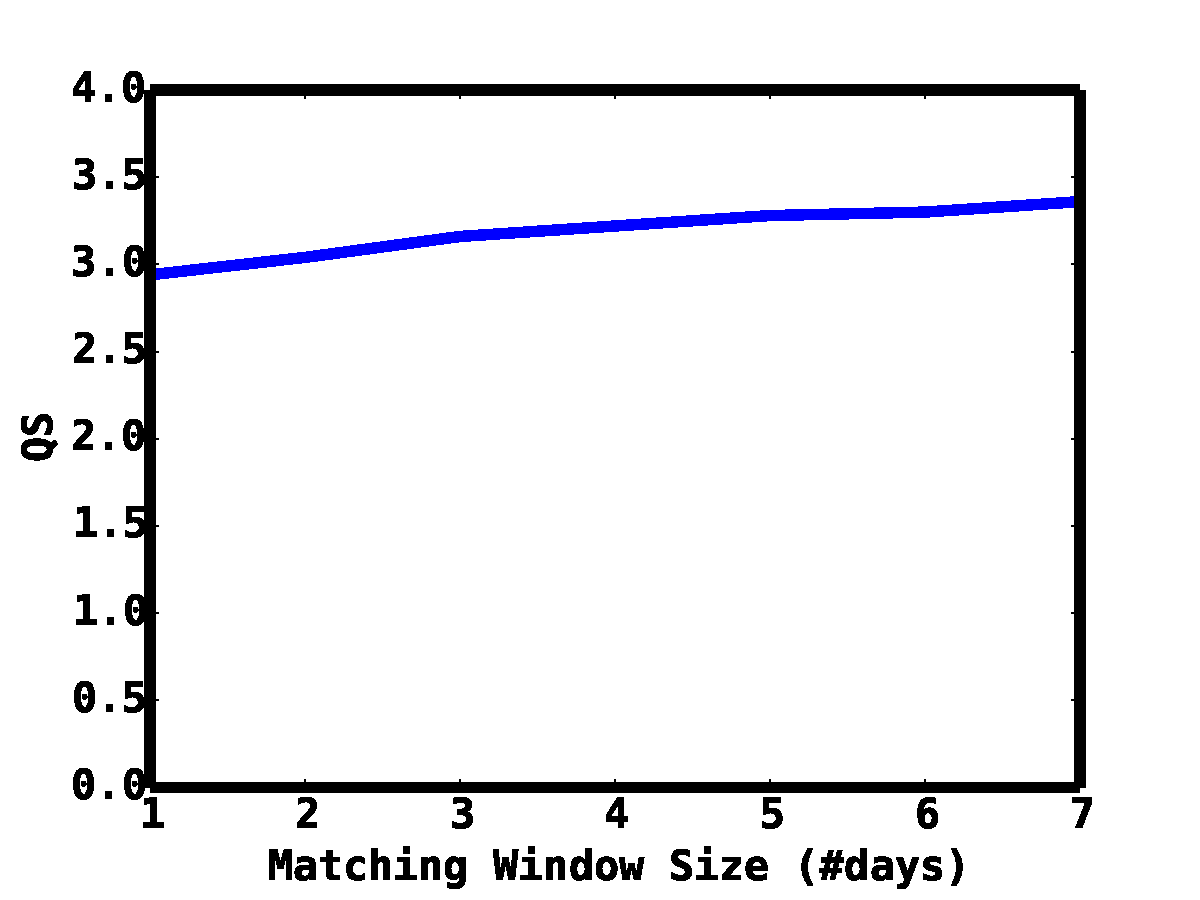
\includegraphics[scale=0.4]{matchingwindow}
    \end{figure}
\end{frame}

\begin{frame}
    \frametitle{Lead-Time vs Quality}
    \begin{figure}
        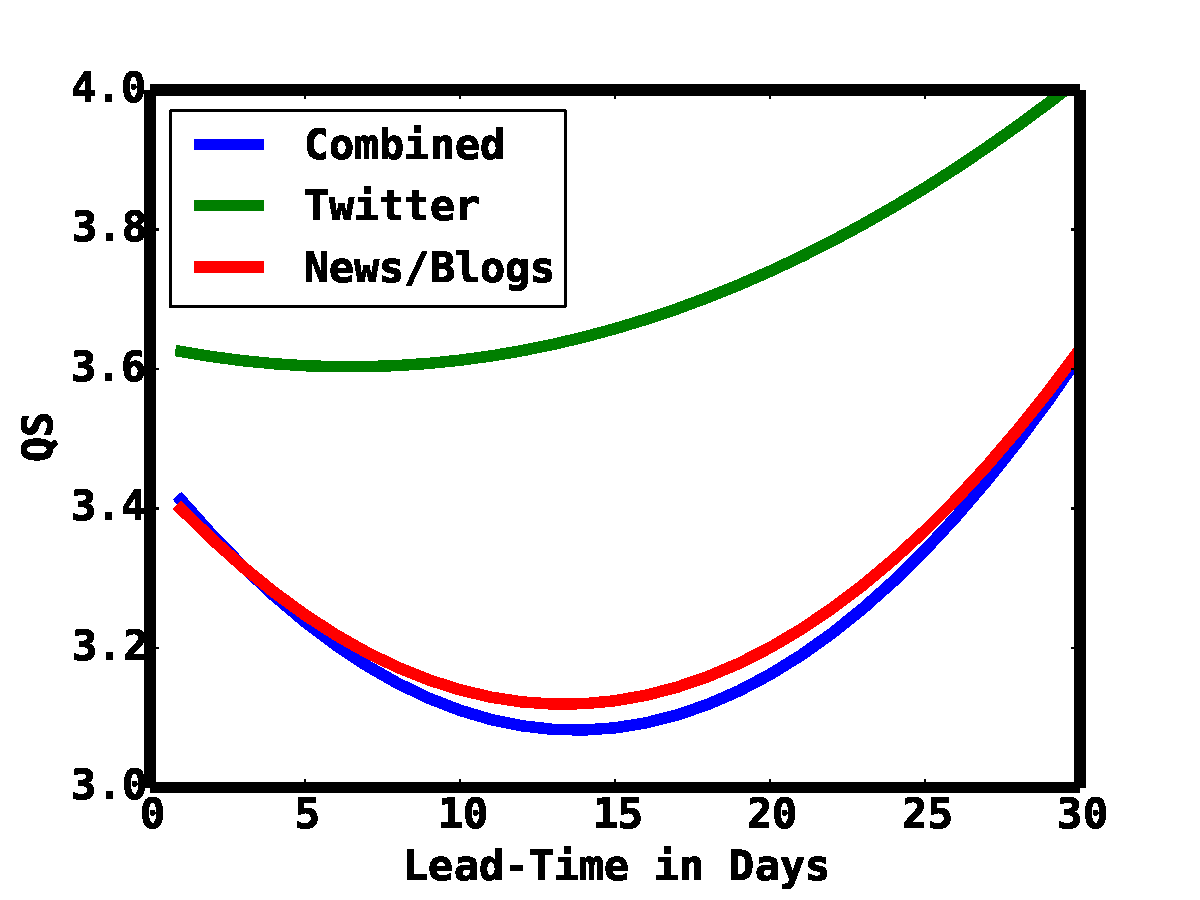
\includegraphics[scale=0.4]{leadTimeVsQS}
    \end{figure}
\end{frame}

\begin{frame}
    \frametitle{Quality Score Distribution}
    \centering
    \begin{figure}
        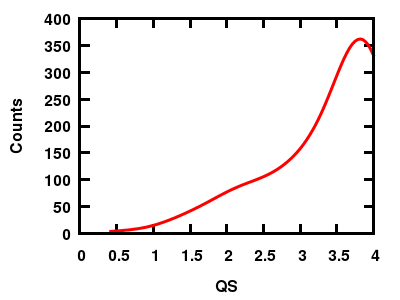
\includegraphics[scale=0.6]{doubleHump}
    \end{figure}
\end{frame}

\begin{frame}
    \frametitle{Conclusion and Framework}
    \begin{itemize}
        \item
            Current system capable of detecting planned protests and resolve $(i)$ date and $(ii)$location of an event satisfactorily
        \item
            Different sources have different advantages and superiorities
        \item
            Future work is aimed at three aspects
            \begin{itemize}
                \item
                    Address situations involving nationwide protests and systems of protests
                \item
                    Generalize system to be able to make predictions from groups of articles and possibly from different sources
                \item
                    Generalize system to detect not-so-explicitly stated expressions of discontent
                \item
                    Generalize approach to consider other population level events of interest other than civil unrest like domestic political crises
                \end{itemize}
        \end{itemize}
\end{frame}

\begin{frame}
    \frametitle{End}
    \center{Thank You!}
\end{frame}

\begin{frame}
    \frametitle{Acknowledgement}
    \center{{\large Acknowledgement}}
\end{frame}


\begin{frame}[noframenumbering]
    \frametitle{Appendix A}
    \begin{itemize}
        \item  Lukasiewicz t-norm
    \begin{figure}
        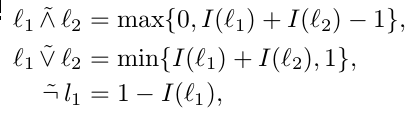
\includegraphics[scale=0.4]{luke_norm}
    \end{figure}
    \item Distance to Satisfaction
    \begin{figure}
        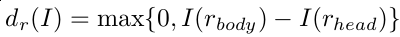
\includegraphics[scale=0.4]{dis_sat_psl}
    \end{figure}
\end{itemize}
\end{frame}
\end{document}
